\documentclass{article}

\usepackage{../preamble}
\standalonetrue

\title{MATH 316 Lecture 11}
\author{Ashtan Mistal}
\date{May 31 2021}

\begin{document}

\ifstandalone
\maketitle
\fi

\graphicspath{{./Lecture11/}}

\section{Introduction}

\begin{itemize}
    \item Check Canvas announcements regarding midterm and such (2 new announcements)
\end{itemize}

\section{Recap of Last Lecture}

Last lecture, we finished up the heat / diffusion equation. 

\begin{itemize}
    \item Homogeneous equations and boundary conditions (Neumann and Dirichlet)
    \item Inhomogeneous equations and boundary conditions
    \item Developed general strategies for splitting inhomogeneous equations into a steady state (Which takes care of inhomogeneous parts, incl. boundary conditions) and a transient part (Satisfying a classic homogeneous diffusion equation)
\end{itemize}

\hfill

Today's lecture is about a new equation: Wave equation. 

Two methods to solve:

\begin{itemize}
    \item Applying separation of variables
    \item We'll talk about the second method tomorrow
\end{itemize}

\section{Wave equation}

Takes the following form:

$$y_{tt} = a^2 y_{xx}$$

Two derivatives with respect to time, and two derivatives with respect to $x$. 

Physically, $a = \left[ \frac{T}{\rho} \right]^{\frac{1}{2}}$ (A string under tension), where $T$ is stress / tension, and $\rho$ is density. Can also be written as $a = \left[ \frac{E}{\rho} \right]^{\frac{1}{2}}$ (Elastic bar), where $E = $ elastic stress. 

Boundary conditions: We have two x derivatives $\to$ 2 conditions needed. 

Initial conditions: We also need 2 initial conditions (Because we have 2 time derivatives). This is the main difference between the wave equation and the heat equation.  $y(x,0) = C$ (Initial displacement), and $y_t(x,0) = k$ (initial velocity)

\hfill

Where did the wave equation come from?

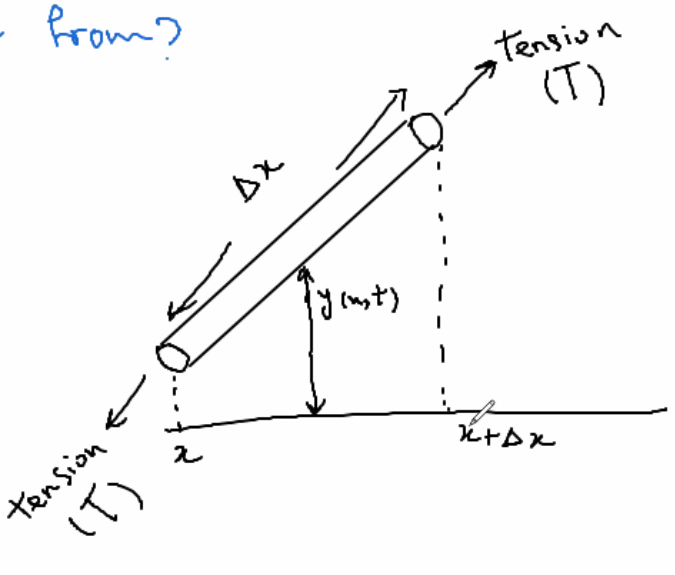
\includegraphics[width = 0.9 \textwidth]{image1.png}

Derivation for small $\left| \frac{\partial y}{\partial x} \right|$

String of density $\rho$ (with units of $\left[ \frac{kh}{m} \right]$)

Force balance in the $y$ direction:

$$\rho \Delta x \frac{\partial^2 y}{\partial t^2} = m \cdot \vec{a} = \sum F_y$$


$$\rho \Delta x \frac{\partial^2 y}{\partial t^2} = T \frac{\partial y}{\partial x} \left( x + \Delta x, t \right) - T \frac{\partial y}{\partial x} (x,t)$$

Divide by $\Delta x$ and let $\Delta x \to 0$:

$$\Rightarrow \rho \frac{\partial^2 y}{\partial t^2} = T \frac{\partial^2 y}{\partial x^2}$$

N.B length of element is $\Delta x (1 + (\frac{\partial y}{\partial x})^2 )^{\frac{1}{2}} \approx \Delta x$

\hfill

\hrule

\hfill

Wave equation: 

$$y_{tt} = a^2 y_{xx}$$

\begin{center}
    BC: $y(0,t) = y(L,t) = 0$
    
    IT: $y(x,0) = f(x)$ and $y_t(x,0) = g(x)$
\end{center}



The idea is to split the solution into two parts. 


\begin{itemize}
    \item Problem 1: Initial velocity, but no displacement of string
    \begin{itemize}
        \item $w_{tt} = a^2 w_{xx}$
        \item $w(0,t) = w(L,t)$
        \item $w(x,0) = 0$ for $0 < x < L$
        \item $w_t(x,0) = g(x)$ for $0 < x < L$
    \end{itemize}
    \item Problem 2: Initial displacement, but no velocity of spring
    \begin{itemize}
        \item $z_{tt} = a^2 z_{xx}$
        \item $z_t (x,0) = f(x)$ for $0 < x < L$
        \item $z_t(x,0) = 0$ for $0 < x < L$
    \end{itemize}
\end{itemize}

Solve problems 1 and 2: $y(x,t) = w(x,t) + z(x,t)$

\subsection{Step 1: Solving Problem 1}

$$w(x,t) = X(x) T(t) \underbrace{\Rightarrow}_{\text{Substitute into PDE}} X \ddot{T} = a^2 X'' T$$

Divide by $a^2 X T$:

$$\Rightarrow \frac{1}{a^2} \frac{\ddot T}{T} = \frac{X''}{X} = - \lambda$$

where $\lambda$ is a constant. 

First, boundary value problem:

$$X'' + \lambda X = 0$$

Boundary conditions are $w(0,t) = X(0) T(t) \Rightarrow X(0) = 0$, and $w(L,t) = X(L) T(t) = 0 \Rightarrow X(L) = 0$

It is a P1 eigenvalue problem. 

Therefore, the eigenvalue problem for $X(x)$ is exactly as for heat / diffusion equation. 

Therefore:

$$\lambda = \lambda_n = \left( \frac{n \pi}{L} \right)^2$$

and $$X_n (x) = \sin \left(\frac{n \pi x}{L} \right)$$

where $n \in \NN$ (Natural numbers; 1,2,3,...)

IVP is:

$$\frac{1}{a^2} \frac{\ddot{T}_n}{T_n} = -\lambda_n \Rightarrow \ddot{T}_n + \left( \frac{a n \pi}{L} \right)^2 T_n = 0$$

Therefore:

$$T_n(t) = A_n \cos \left(\frac{a n \pi}{L} t \right) + B_n \sin \left(\frac{a n \pi}{L} t \right)$$

How about the initial condition?

$w(x,0) = 0 \longrightarrow X(x) T(0) = 0 \Rightarrow T(0) = 0$ and $w_t (x,0) = g(x)$

$T_n (0) = 0 \Rightarrow A_n = 0$

\hfill

As a result:

$$T_n(t) = B_n \sin \left(\frac{a n \pi}{L} t \right)$$

Now, note that PDE, boundary conditions, and $w(x,0)$ are homogeneous. Therefore, we can superimpose solutions. 

$$w(x,t) = \sum_{n = 1}^\infty B_n \sin \left(\frac{n \pi x}{L} \right) \sin \left(\frac{a n \pi}{L} t \right)$$

We need to find $B_n$. To find this, we use the second initial condition. 

$$w_t (x,0) = \sum_{n = 1}^\infty B_n \left(\frac{a n \pi}{L} \right)  \sin \left(\frac{n \pi x}{L} \right) \cos \left(\frac{a n \pi}{L} t \right)$$

$$w_t (x,0) = \sum_{n = 1}^\infty B_n \left(\frac{a n \pi}{L} \right) \sin \left( \frac{n \pi x}{L} \right) = g(x)$$

If we write a Fourier sine series for $g(x)$, we can match up the coefficients:

To make this work, represent $g(x)$ as a Fourier sine series on $\left[ 0, L \right]$:

$$g(x) = \sum_{n = 1}^\infty b_n \sin \left(\frac{ n \pi x}{L} \right) \Rightarrow b_n = \frac{2}{L} \int_0^L g(x) \sin \left( \frac{ n \pi x}{L} \right) dx$$

We know this series converges, so we match up the coefficients. 
\begin{center}
    $B_n = b_n \frac{L}{n \pi a}$ for $n \in \NN$. 
\end{center}


$$\Rightarrow w(x,t) = \sum_{n = 1}^\infty b_n \frac{L}{n \pi a} \sin \left( \frac{n \pi x}{L} \right) \sin \left( \frac{n \pi a t}{L} \right) $$

\subsection{Step 2: Solving Problem 2}

$$z_{tt} = a^2 z_{xx}$$

Initial boundary conditions: $z(0,t) = Z(L,t) = 0$ and $Z(x,0) = f(x)$; $z_t (x,0) = 0$ for $0 < x < L$

Solution: Similarly, we use separation of variables and we assume that $z$ is a product of $X$ and $T$:

$$z(x,t) = X(x) T(t)$$

(Note that these are different X and T than in step 1!!)

The solution for the eigenvalue problem is a P1 problem again. 

$$X_n(x) = \sin \left( \frac{n \pi x}{L} \right)$$
\begin{center}
    $\lambda_n = \left( \frac{n \pi}{L} \right)^2$ for $n \in \NN$
\end{center}


For the IVP part, 

$$\ddot{T}_n + \left( \frac{n \pi a}{L} \right)^2 T_n = 0$$

$$\Rightarrow T_n(t) = A_n \cos \left( \frac{n \pi a}{L} t \right) + B_n \sin \left( \frac{n \pi a}{L} t \right)$$

Now, $z_t(x,0) = X(x) \dot{T}(0) = 0 \Rightarrow \dot{T}_n(0) = 0 \Rightarrow B_n = 0$

So, let's superimpose the solution:

$$z_n (x,t) = \sum_{n = 1}^\infty A_n \sin \left( \frac{n \pi x}{L} \right) \cos \left( \frac{n \pi a}{L} t \right)$$

Use the other initial condition and find $A_n$:

The other initial condition tells us:

$$f(x) = z(x,0) = \sum_{n =1}^\infty  A_n \sin \left( \frac{n \pi x}{L} \right)$$

Suppose we compute the Fourier sine series for $f(x)$, Then, $$b_n' = \frac{2}{L} \int_0^L f(x) \sin \left( \frac{n \pi x}{L} \right) dx$$

\textbf{Note that prime is NOT a derivative, just used to denote that it's a different} $b_n$.

$$\Rightarrow z(x,t) = \sum_{n = 1}^\infty b_n' \sin \left( \frac{n \pi x}{L} \right) \cos \left( \frac{n \pi a}{L} t \right)$$

\subsection{Step 3}

$$y(x,t) = x(x,t) + z(x,t)$$

$$ y(x,t) = \sum_{n = 1}^\infty \left[ b_n \frac{L}{n \pi a} \sin \left( \frac{n \pi x}{L} \right) \sin \left( \frac{n \pi a t}{L} \right) + b_n' \sin \left( \frac{n \pi x}{L} \right) \cos \left( \frac{n \pi a}{L} t \right) \right]$$

We can factor\footnote{Again, $b_n'$ is not a derivative!}:

$$y(x,t) = \sum_{n = 1}^\infty \sin \left( \frac{n \pi x}{L} \right) \left[ \frac{b_n L}{n \pi a} \sin \left( \frac{n \pi a}{L}  t \right) + b_n' \cos \left( \frac{n \pi a}{L}  t \right) \right]$$

\hfill

For Neumann boundary conditions, the procedure is exactly the same as Dirichlet boundary conditions. 

(Using the PDF file posted on Canvas -- Wave Equations, under week 4. Posted at the bottom of this document.)

\section{Example 8}

(Example 8 of the pdf)

Solve the IBVP $y_{tt} = y_{xx}$

Initial conditions: $y(0,t) = y(2,t)$

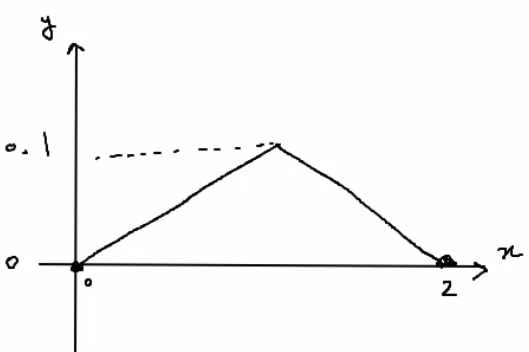
\includegraphics[width = 0.8 \textwidth]{image2.png}

$y(x,0) = \left\{ \begin{matrix} 0.1 x & 0 \leq x \leq 1 \\ 0.1(2-x) & 1 \leq x \leq 1 \end{matrix} \right.$

$y_t (x,0) = 0 = g(x) \Rightarrow b_n = 0$ $ \forall n$

Solution: a = 1 and L = 2. (There is only initialdisplacement $z(x,t)$ problem)

$$b_n' = \frac{2}{L} \int_0^L g(x) \sin \left( \frac{ n \pi x}{L} \right) dx = 0.1 \int_0^1 x \sin \left( \frac{ n \pi x}{2} \right) + 0.1\int_1^2 (2-x) \sin \left( \frac{ n \pi x}{2} \right) $$

$$b_n' = - \frac{0.2}{n \pi} \cos \left( \frac{n \pi}{2} \right) + 0 + \frac{0.4}{(n \pi)^2 } \cdot \left. \sin \left( \frac{n \pi x}{2} \right) \right|_0^1  - 0 + \frac{0.2}{n \pi} \cos( \frac{n \pi}{2}) - \frac{0.4}{(n \pi)^2} \left. \sin  \left( \frac{n \pi x}{2} \right) \right|_1^2$$

$$b_n' = \frac{0.8}{(n \pi)^2 } \sin \left( \frac{n \pi}{2} \right)$$


$$y(x,t) = \sum_{n = 1}^\infty \frac{0.8}{(n \pi)^2 } \sin \left( \frac{n \pi}{2} \right) \sin \left( \frac{n \pi x}{2} \right) \cos \left( \frac{n \pi}{2} t \right)$$

N.B\footnote{Nota bene. Used to denote an important point. }:

$\sin (\frac{n \pi}{2}) = 1,0,-1,0,1,0,...$ for $n \in \NN$

Thus, we could write $n = 2k-1$ and $b_k' = (-1)^{k+1}$ for $k \in \NN$

$$y(x,t) = \sum_{k  =1}^\infty \frac{0.8 (-1)^{k + 1}}{(2k-1)^2 \pi^2} \sin \left( \frac{(2k-1) \pi}{2} x \right) \cos \left( \frac{(2k-1) \pi}{2} t \right)$$

\section{Example 9}

$$y_{tt} = y_{xx}$$

$y(0,t) = 0$ and $y(1,t) = 0$

$y(x,0) = 0$ and $y_t(x,0) = \sin(5 \pi x)$

Solution: a = 1 and L = 1 and $f(x) = 0$ $\Rightarrow$ we only have the velocity problem to solve. 

Need to find the Fourier sine series for $g(x)$:

$$\sum_{n  =1}^\infty b_n \sin(n \pi x) = g(x) = \sin(5 \pi x)$$

But this is already a fourier series. For any $n$ value $\neq 5$, $b_n = 0$. $b_5 = 1$. 

Therefore, the general solution 

$$y(x,t) = \frac{1}{5 \pi} \sin (5 \pi x) \sin(5 \pi t)$$

\section{Wave Equations PDF}

Wave Equations PDF is removed in exports to save space but is available in the source code. 

%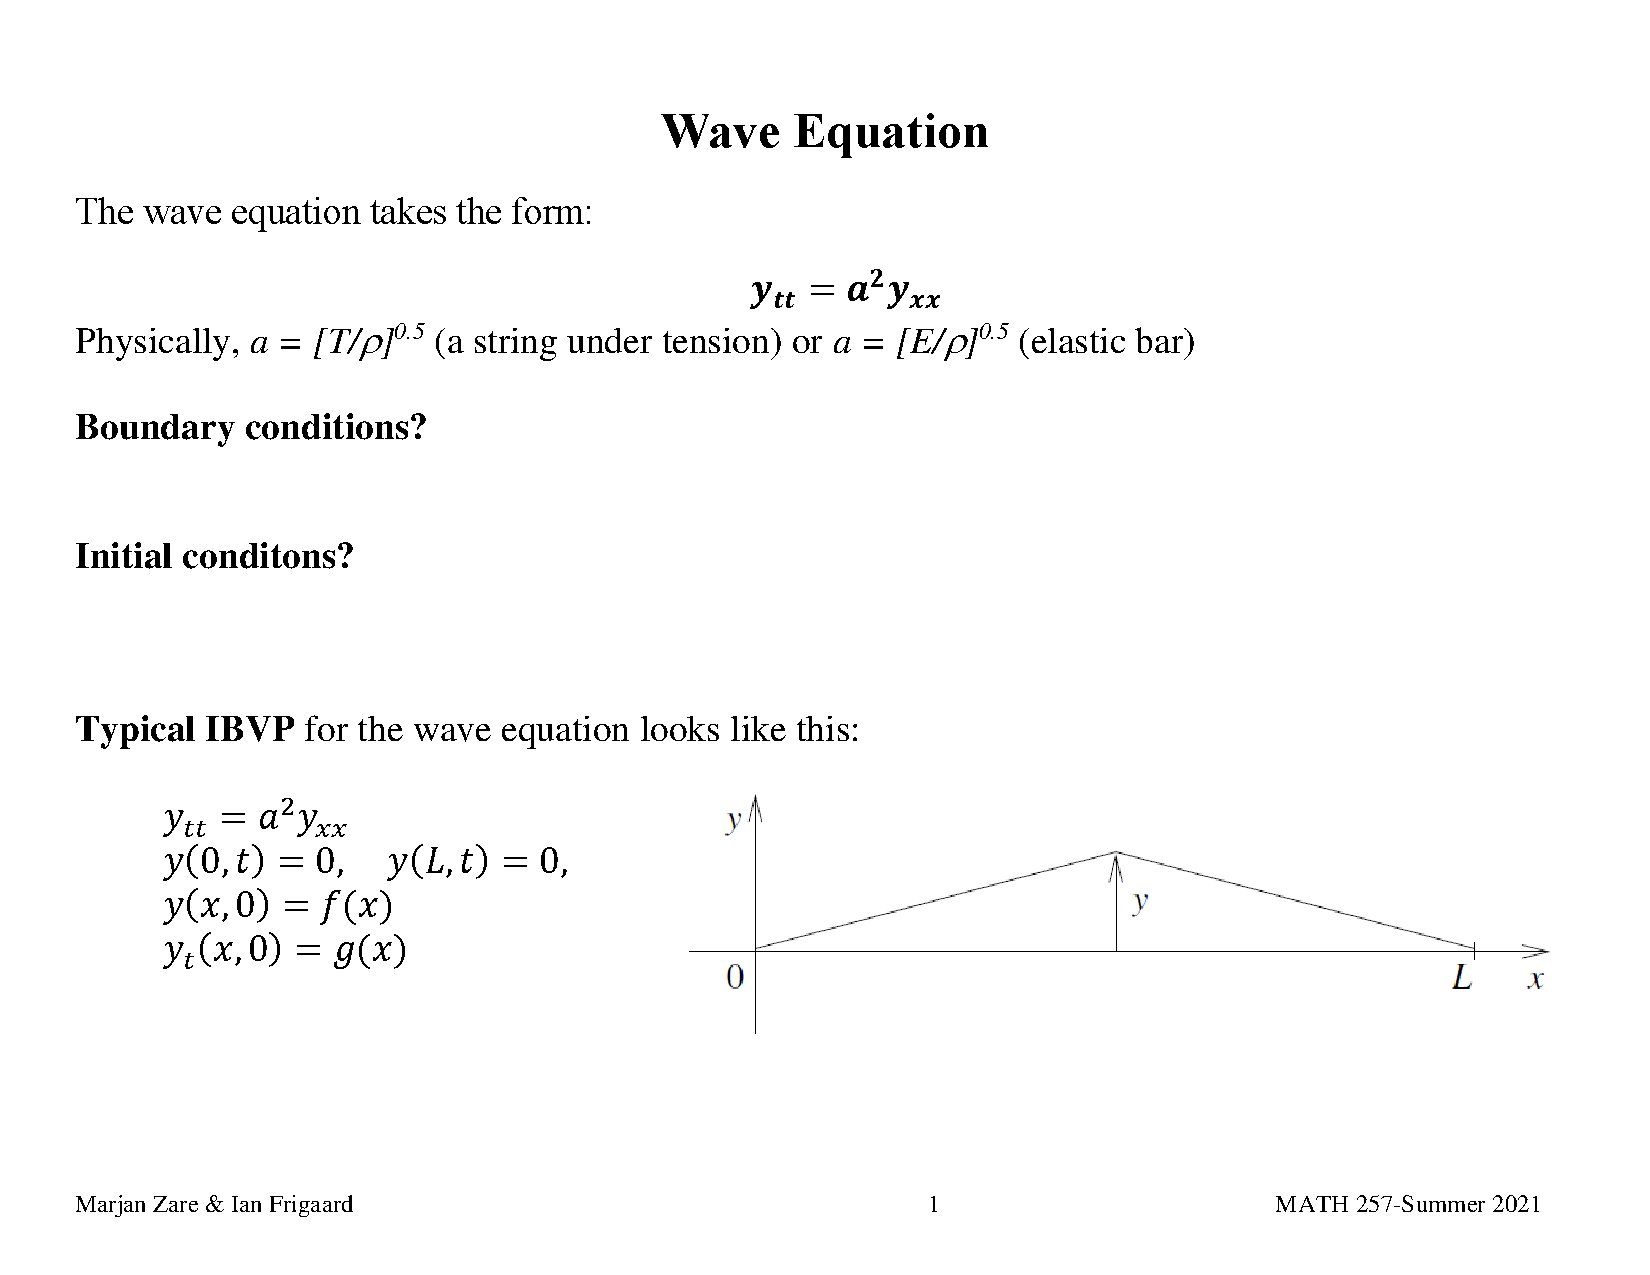
\includepdf[pages=-]{Wave_Equations.pdf}

\end{document}